\documentclass{article}
\usepackage{lmodern}
\usepackage[T1]{fontenc}
\usepackage{shapepar}
\usepackage{microtype}
\usepackage{lipsum}
\usepackage{pgfplots}
\pgfplotsset{compat=1.9}
\usepackage{tikz}
\usetikzlibrary{calc,fit,intersections,folding}
\usepackage{pstricks-add}
\usetikzlibrary{arrows.meta,angles,arrows,quotes,backgrounds}
\usepackage[a3paper,left=5mm,right=5mm,top=25mm,bottom=25mm]{geometry} % Ränder

\begin{document}
\thispagestyle{empty}
    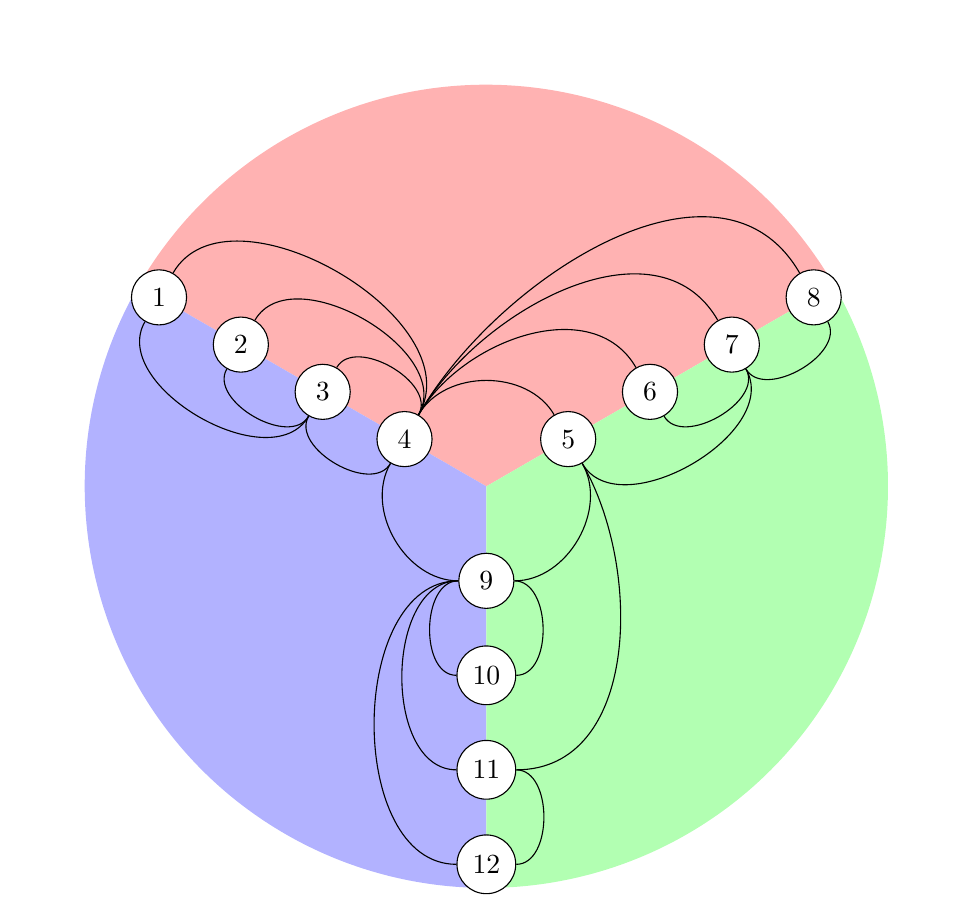
\begin{tikzpicture}[scale = 0.6]
        \node[draw,fill=white,minimum size =7mm] (A) at (30:2cm) [circle] {5};
        \node[draw,fill=white,minimum size =7mm] (B) at (30:4cm) [circle] {6};
        \node[draw,fill=white,minimum size =7mm] (C) at (30:6cm) [circle] {7};
        \node[draw,fill=white,minimum size =7mm] (D) at (30:8cm) [circle] {8};

        \node[draw,fill=white,minimum size =7mm] (a) at (150:2cm) [circle] {4};
        \node[draw,fill=white,minimum size =7mm] (b) at (150:4cm) [circle] {3};
        \node[draw,fill=white,minimum size =7mm] (c) at (150:6cm) [circle] {2};
        \node[draw,fill=white,minimum size =7mm] (d) at (150:8cm) [circle] {1};
        
        \node[draw,fill=white,minimum size =7mm] (w) at (270:2cm) [circle] {9};
        \node[draw,fill=white,minimum size =7mm] (x) at (270:4cm) [circle] {10};
        \node[draw,fill=white,minimum size =7mm] (y) at (270:6cm) [circle] {11};
        \node[draw,fill=white,minimum size =7mm] (z) at (270:8cm) [circle] {12};

        \draw (A) to[out = -60, in = 0]     (w);
        \draw (A) to[out = -60, in = 0]     (y);
        \draw (A) to[out = -60, in = -60]   (C);
        \draw (B) to[out = -60, in = -60]   (C);
        \draw (C) to[out = -60, in = -60]   (D);
        \draw (w) to[out = 0  , in = 0]     (x);
        \draw (y) to[out = 0  , in = 0]     (z);

        \draw (a) to[out = 60, in = 120]    (A);
        \draw (a) to[out = 60, in = 120]    (B);
        \draw (a) to[out = 60, in = 120]    (C);
        \draw (a) to[out = 60, in = 120]    (D);
        \draw (a) to[out = 60, in = 60]     (b);
        \draw (a) to[out = 60, in = 60]     (c);
        \draw (a) to[out = 60, in = 60]     (d);

        \draw (w) to[out = 180, in = 180]   (x);
        \draw (w) to[out = 180, in = 180]   (y);
        \draw (w) to[out = 180, in = 180]   (z);
        \draw (w) to[out = 180, in = 240]   (a);
        \draw (a) to[out = 240, in = 240]   (b);
        \draw (b) to[out = 240, in = 240]   (c);
        \draw (b) to[out = 240, in = 240]   (d);
        

         \begin{scope}[on background layer]
             \fill[red!30!white] (0,0) -- (30:8.5cm) arc (30:150:8.5cm) -- (0,0);
             \fill[blue!30!white] (0,0) -- (150:8.5cm) arc (150:270:8.5cm) -- (0,0);
             \fill[green!30!white] (0,0) -- (30:8.5cm) arc (30:-90:8.5cm) -- (0,0);
         \end{scope}
    \end{tikzpicture}
\end{document}
